 \chapter{机械振子：阻尼与共振}\label{ch:b1:oscillators-resonance}

在错误的时刻推小孩的秋千，几乎没有效果；
若每个周期轻轻推一次，不出十二次摆动，孩子
就会在摆动的最高处尖叫起来。洗衣机甩干时，若转速
恰好处于某一特定值，就会剧烈抖动，高于此转速则安静下来。
湿手指以恰当的速率沿酒杯杯口画圈，酒杯便会发出声音；
歌唱者若以足够大的音量唱出同一音高，酒杯甚至会被震碎。
这些现象都是\emph{共振}：一个具有固有频率的系统，
在该频率附近受到驱动时，能量会逐周累积，
直到摩擦力耗散能量的速率与输入能量的速率相当为止。本章
研究机械振子——依次为自由振子、阻尼振子和受迫振子——
并推导共振曲线，其电学对应物
已在\cref{ch:b1:sinusoidal-impedance}中出现。

\section{谐振子}

\begin{definition}[谐振子]\label{def:b1:oscillators-resonance:harmonic}
\index{谐振子}\index{固有频率}
若一系统相对于稳定平衡位置的位移 $x$ 满足
\[
\ddot x + \omega_0^2\,x = 0
\]
则称其为\emph{谐振子}，其\emph{固有角频率}
$\omega_0$（周期 $T_0 = 2\pi/\omega_0$）。方程的解 $x = A\cos(\omega_0t
+ \varphi)$ 的振幅和相位由初始条件确定，
而周期与振幅无关（\emph{等时性}）。
\end{definition}

\begin{proposition}[谐振子的来源]\label{prop:b1:oscillators-resonance:sources}
\begin{itemize}
  \item 质量为 $m$ 的物体系于劲度系数为 $k$ 的弹簧上：$\omega_0^2 = k/m$（胡克定律）。
  \item 长为 $\ell$ 的单摆（小角度近似）：$\omega_0^2 = g/\ell$。
  \item 位于势能 $E_p$ 稳定平衡点附近的任意质点：
        $\omega_0^2 = E_p''(x_0)/m$（\cref{prop:b1:work-and-energy:stability}）。
  \item LC 电路：$\omega_0^2 = 1/LC$，并取 $q \leftrightarrow x$，
        $L \leftrightarrow m$，$1/C \leftrightarrow k$。
\end{itemize}
能量 $E = \tfrac12 m\dot x^2 + \tfrac12 m\omega_0^2x^2 = \tfrac12
m\omega_0^2A^2$ 为常量，在动能与势能两种形式之间
每个周期来回转换两次。
\end{proposition}

\begin{proof}
由牛顿第二定律并取 $F = -kx$；单摆方程
$\ddot\theta + (g/\ell)\sin\theta = 0$，取 $\sin\theta \approx \theta$；
在 $E_p$ 的极小值处用泰勒公式；LC 电路的
回路定律。能量：对其求导并利用运动方程。
\end{proof}

\begin{example}[上下浮动的圆柱体]\label{ex:b1:oscillators-resonance:bob}
竖直放置的圆柱体，横截面积为 $S$，漂浮时
浸入深度为 $h$（$mg = \rho_wgSh$，浮力见\cref{ch:b1:fluid-statics}）。
向下压 $x$ 后，它受到额外的向上力 $\rho_wgSx$：
$m\ddot x = -\rho_wgSx$，故 $\omega_0^2 = \rho_wgS/m = g/h$——与
长为 $h$ 的单摆相同。浸入深度为 \qty{1}{m} 的浮标，
上下浮动，周期为 \qty{2}{s}，与其质量无关。
\end{example}

\section{阻尼振子}

\begin{proposition}[阻尼振子]\label{prop:b1:oscillators-resonance:damped}
\index{阻尼振子}\index{品质因数!机械}
若存在黏性摩擦力 $-\alpha\dot x$，方程变为
\[
\ddot x + \frac{\omega_0}{Q}\dot x + \omega_0^2x = 0, \qquad
Q = \frac{\sqrt{km}}{\alpha} = \frac{m\omega_0}{\alpha},
\]
这是\cref{ch:b1:transient-regimes}中的标准二阶形式。当
$Q > \tfrac12$ 时，为准周期衰减 $x = A\eu^{-t/\tau}\cos(\omega t +
\varphi)$，其中 $\tau = 2Q/\omega_0$，$\omega = \omega_0\sqrt{1 - 1/4Q^2}$；
能量按 $\eu^{-2t/\tau}$ 衰减，且
\[
Q = 2\pi\,\frac{\text{储存的能量}}{\text{每周期损失的能量}}
\quad (Q \gg 1) .
\]
\end{proposition}

\begin{proof}
将 $m\ddot x + \alpha\dot x + kx = 0$ 除以 $m$。对能量，$E
\propto A^2\eu^{-2t/\tau}$，每周期损失的比例为 $2T/\tau = 2\pi/Q$
（在该值较小时成立）。
\end{proof}

\begin{example}[余音时长]\label{ex:b1:oscillators-resonance:ringing}
一个频率为 \qty{440}{Hz} 的音叉，
被敲击后十秒仍在发声：其振幅降至约 $5\%$，所用时间为 $3\tau = \qty{10}{s}$，
因此 $\tau = \qty{3.3}{s}$，且 $Q = \omega_0\tau/2 \approx 4600$。汽车的
悬架（$Q \approx 0.7$）在一个周期内即停止振动；小孩的秋千
（$Q \approx 20$）每次摆动损失三分之一的能量，
因而每次都需要推一把。
\end{example}

\section{受迫振动与共振}

\begin{theorem}[正弦驱动振子]\label{thm:b1:oscillators-resonance:forced}
\index{受迫振动}\index{共振!振幅}\index{共振!速度}
在力 $F_0\cos\omega t$ 的驱动下，阻尼振子
\[
m\ddot x + \alpha\dot x + kx = F_0\cos\omega t
\]
经过持续时间 $\sim\tau$ 的暂态后，振子进入
受迫稳态 $x = X\cos(\omega t + \varphi)$，其中记 $x_r = \omega/\omega_0$
及 $X_0 = F_0/k$ 为静态位移，则
\[
X = \frac{X_0}{\sqrt{(1 - x_r^2)^2 + x_r^2/Q^2}}, \qquad
\tan\varphi = -\frac{x_r/Q}{1 - x_r^2}, \quad \varphi \in [-\pi, 0] .
\]
\emph{振幅} $X$ 在 $Q > 1/\sqrt2$ 时，于 $\omega_r =
\omega_0\sqrt{1 - 1/2Q^2}$ 处达到峰值，且 $X_{\max} \approx QX_0$；\emph{速度
振幅} $V = \omega X$ 恰在 $\omega_0$ 处达到峰值，其中 $V_{\max} =
F_0/\alpha$，其共振曲线为
\[
\frac{V}{V_{\max}} = \frac{1}{\sqrt{1 + Q^2(x_r - 1/x_r)^2}}
\]
带宽为 $\Delta\omega = \omega_0/Q$。在 $\omega_0$ 处，位移
滞后于力 $\pi/2$，速度则与力同相。
\end{theorem}

\begin{proof}
用复数法（见\cref{ch:b1:sinusoidal-impedance}）：$\underline X(-\omega^2
+ j\omega\omega_0/Q + \omega_0^2) = F_0/m$，于是 $\underline X = (F_0/m)/(\omega_0^2
- \omega^2 + j\omega\omega_0/Q)$；分子与分母同除以
$\omega_0^2 = k/m$。模与辐角随之可得；$X$ 的最大值
已在\cref{prop:b1:sinusoidal-impedance:overvoltage}中求出，
二者为同一函数。速度：由 $\underline V = j\omega\underline X$ 得 $V = \omega X$；
将 $(1 - x_r^2)/x_r = 1/x_r - x_r$ 代入，分母化为
$\sqrt{1/Q^2 + (1/x_r - x_r)^2}$，即 RLC 形式。当 $x_r = 1$ 时，
$\underline X = -jQX_0$，滞后 $\pi/2$。
\end{proof}

\begin{omfigure}
\begin{tikzpicture}
\begin{axis}[omaxis, width=7.6cm, height=5.6cm, xlabel={$\omega/\omega_0$}, ylabel={$X/X_0$},
    xmin=0, xmax=2.1, ymin=0, ymax=5.8, xtick={0.5,1,1.5,2}, ytick={1,2,3,4,5},
    legend style={at={(0.97,0.97)}, anchor=north east, font=\footnotesize, draw=none, fill=none}]
  \addplot[omThm, thick, domain=0:2.1, samples=400] {1/sqrt((1-x^2)^2 + x^2/25)};
  \addlegendentry{$Q = 5$}
  \addplot[omDef, thick, domain=0:2.1, samples=300] {1/sqrt((1-x^2)^2 + x^2/4)};
  \addlegendentry{$Q = 2$}
  \addplot[omProp, thick, domain=0:2.1, samples=300] {1/sqrt((1-x^2)^2 + 2*x^2)};
  \addlegendentry{$Q = 1/\sqrt2$}
  \addplot[omProp!60!black, thick, domain=0:2.1, samples=300] {1/sqrt((1-x^2)^2 + x^2/0.09)};
  \addlegendentry{$Q = 0.3$}
\end{axis}
\end{tikzpicture}\qquad
\begin{tikzpicture}
\begin{axis}[omaxis, axis x line=bottom, width=7.0cm, height=5.6cm, xlabel={$\omega/\omega_0$}, ylabel={$\varphi$},
    xmin=0, xmax=2.1, ymin=-3.4, ymax=0.4, xtick={0.5,1,1.5,2}, ytick={-3.1416,-1.5708,0},
    yticklabels={$-\pi$,$-\frac{\pi}{2}$,$0$}]
  \addplot[omThm, thick, domain=0:0.999, samples=200] {-atan((x/5)/(1-x^2))*pi/180};
  \addplot[omThm, thick, domain=1.001:2.1, samples=200] {-pi - atan((x/5)/(1-x^2))*pi/180};
  \addplot[omDef, thick, domain=0:0.999, samples=200] {-atan((x/2)/(1-x^2))*pi/180};
  \addplot[omDef, thick, domain=1.001:2.1, samples=200] {-pi - atan((x/2)/(1-x^2))*pi/180};
  \addplot[omProp!60!black, thick, domain=0:0.999, samples=200] {-atan((x/0.3)/(1-x^2))*pi/180};
  \addplot[omProp!60!black, thick, domain=1.001:2.1, samples=200] {-pi - atan((x/0.3)/(1-x^2))*pi/180};
\end{axis}
\end{tikzpicture}

{\small 受迫振子的振幅（左）与相位（右）
随驱动频率的变化，取若干品质因数。尖锐的
峰出现在 $\omega_0$ 附近（$Q$ 较大时），$Q = 1/\sqrt2$ 以下则无峰；位移
由低频（$\omega$ 小）时的同相变为
高频（$\omega$ 大）时的反相，途经 $\pi/2$ 滞后（在 $\omega_0$ 处）——共振越尖锐，
相位转换越急剧。}
\end{omfigure}

\begin{remark}[两种共振，一个电路]\label{rem:b1:oscillators-resonance:analogy}
\index{机电类比}
对应关系为 $x \leftrightarrow q$，$\dot x \leftrightarrow i$，
$m \leftrightarrow L$，$\alpha \leftrightarrow R$，$k \leftrightarrow 1/C$，
$F \leftrightarrow e$，将受迫振子映射为
在\cref{ch:b1:sinusoidal-impedance}中的串联 RLC 电路：速度共振即
电流共振（总在 $\omega_0$ 处，带宽 $\omega_0/Q$），振幅
即电荷共振，亦即电容器电压的共振（略
低于 $\omega_0$，低 $Q$ 时不出现）。吸收功率 $\langle F\dot x\rangle
= \tfrac12 F_0V\cos\varphi_v$，在 $\omega_0$ 处达到峰值 $F_0^2/2\alpha$，
而半功率点即为速度带宽，与
RLC 电路完全一致。
\end{remark}

\begin{example}[共振速率]\label{ex:b1:oscillators-resonance:road}
某汽车悬架的 $f_0 \approx \qty{1.3}{Hz}$（见\cref{pb:b1:transient-regimes:1}）。
若路面每隔 $\lambda = \qty{10}{m}$ 有一道起伏，则激励
频率为 $v/\lambda$：当 $v = \lambda f_0 = \qty{13}{m/s}$ 时发生共振，
约 \qty{47}{km/h}——此时搓衣板式路面
使车身振动最剧烈，这也是装设 $Q \approx 0.7$ 减振器的原因：
若 $Q = 5$，车身振动的
振幅将是路面振幅的五倍。高于共振（$x_r \gg 1$）时，振幅按
$X_0/x_r^2$ 下降：车身在快速颠簸上“悬浮”——隔振，
是共振的另一面。
\end{example}

\section{基座激励：隔振与地震仪}

\begin{proposition}[由支座带动的振子]\label{prop:b1:oscillators-resonance:base}
\index{基座激励}\index{隔振}\index{地震仪}
设质量–弹簧–阻尼器系统的支座发生位移 $x_g(t)$（如汽车下的路面、
地震仪下的地面），设 $u$ 为质量相对于支座的
位移，$x = x_g + u$ 为其绝对位移（自
平衡位置算起）。则
\[
m\ddot u + \alpha\dot u + ku = -m\ddot x_g ,
\]
当 $x_g = X_g\cos\omega t$，且 $x_r = \omega/\omega_0$ 时：
\[
\frac{U}{X_g} = \frac{x_r^2}{\sqrt{(1 - x_r^2)^2 + x_r^2/Q^2}},
\qquad
\frac{X}{X_g} = \sqrt{\frac{1 + x_r^2/Q^2}{(1 - x_r^2)^2 + x_r^2/Q^2}} .
\]
当 $x_r \gg 1$ 时，$U \to X_g$（质量在空间中保持静止——
\emph{地震仪}由此读出地面的位移）且 $X \to 0$（质量
被\emph{隔离}于振动之外）；当 $x_r \ll 1$ 时，$U \approx
\ddot x_g/\omega_0^2$（\emph{加速度计}）且 $X \approx X_g$（质量
随支座运动）。
\end{proposition}

\begin{proof}
弹簧与阻尼器作用于相对运动：$m\ddot x = -ku -
\alpha\dot u$，又 $\ddot x = \ddot x_g + \ddot u$。取复数形式，
$\underline U(\omega_0^2 - \omega^2 + j\omega\omega_0/Q) = \omega^2X_g$，由此得
$U/X_g$；进而 $\underline X = \underline U + X_g = X_g(1 + jx_r/Q)/(1 -
x_r^2 + jx_r/Q)$。
\end{proof}

\begin{omfigure}
\begin{tikzpicture}
\begin{axis}[omaxis, axis x line=bottom, axis y line=left, xlabel style={at={(axis description cs:0.5,-0.14)}, anchor=north},
    width=7.4cm, height=5.4cm, xmode=log, ymode=log, xlabel={$\omega/\omega_0$}, ylabel={$U/X_g$},
    xmin=0.1, xmax=10, ymin=0.005, ymax=10, xtick={0.1,1,10}, xticklabels={$0.1$,$1$,$10$},
    ytick={0.01,0.1,1,10}, yticklabels={$0.01$,$0.1$,$1$,$10$},
    legend style={at={(0.03,0.97)}, anchor=north west, font=\footnotesize, draw=none, fill=none}]
  \addplot[omThm, thick, domain=0.1:10, samples=300] {x^2/sqrt((1-x^2)^2 + x^2/25)};
  \addlegendentry{$Q = 5$}
  \addplot[omDef, thick, domain=0.1:10, samples=300] {x^2/sqrt((1-x^2)^2 + 2*x^2)};
  \addlegendentry{$Q = 1/\sqrt2$}
  \node[font=\footnotesize, anchor=west] at (axis cs:1.6,0.05) {地震仪};
  \node[font=\footnotesize, anchor=west] at (axis cs:0.2,0.018) {加速度计};
\end{axis}
\end{tikzpicture}\qquad
\begin{tikzpicture}
\begin{axis}[omaxis, axis x line=bottom, axis y line=left, xlabel style={at={(axis description cs:0.5,-0.14)}, anchor=north},
    width=7.0cm, height=5.4cm, xmode=log, ymode=log, xlabel={$\omega/\omega_0$}, ylabel={$X/X_g$},
    xmin=0.1, xmax=10, ymin=0.005, ymax=10, xtick={0.1,1,10}, xticklabels={$0.1$,$1$,$10$},
    ytick={0.01,0.1,1,10}, yticklabels={$0.01$,$0.1$,$1$,$10$}]
  \addplot[omThm, thick, domain=0.1:10, samples=300] {sqrt((1 + x^2/25)/((1-x^2)^2 + x^2/25))};
  \addplot[omDef, thick, domain=0.1:10, samples=300] {sqrt((1 + 2*x^2)/((1-x^2)^2 + 2*x^2))};
  \node[font=\footnotesize, anchor=west] at (axis cs:1.8,2.0) {隔振};
\end{axis}
\end{tikzpicture}

{\small 一个经其支座摇动的质量块。左图：相对运动
$U/X_g$——低于 $\omega_0$ 时为加速度计（对数坐标上斜率为 $2$），
高于该频率时为地震仪。右图：绝对运动 $X/X_g$——质量块
低频时随支座运动，远高于
$\omega_0$ 时则与之隔离；高 $Q$ 值毫无益处，只会产生危险的峰值。}
\end{omfigure}

\begin{example}[为什么机器要装在软垫座上]\label{ex:b1:oscillators-resonance:mounts}
一台 \qty{50}{Hz} 的电动机装在调谐至 $f_0 = \qty{10}{Hz}$ 的橡胶垫座上，
（$x_r = 5$，$Q \approx 2$）：$X/X_g = \sqrt{(1 + 6.25)/(576 + 6.25)} = 0.11$，
即约九成的振动被隔绝在地面之外。垫座必须
比直觉所认为的更\emph{软}：若将其加固，$f_0$
升至接近 $50$ Hz，隔振效果随之丧失。同一公式反过来读，
便是 \cref{ex:b1:oscillators-resonance:road} 中的汽车在
搓板路上行驶时的情形。
\end{example}

\section{能量：共振如何积累}

\begin{proposition}[受迫状态下的能量平衡]\label{prop:b1:oscillators-resonance:energy}
在稳态受迫振动中，驱动力提供的平均功率
等于摩擦力耗散的平均功率，$\tfrac12\alpha V^2$。
共振时，储存能量 $\tfrac12 mV_{\max}^2$ 为每周期所提供能量的
$Q/2\pi$ 倍：振子在约
$Q$ 个循环内累积驱动力所做的功，直到损耗与输入相等；这也是
暂态持续的循环数（$\sim\tau/T$）。
\end{proposition}

\begin{proof}
对一个周期取能量定理的平均：$\langle\dd E/\dd t\rangle = 0$
稳态下，故 $\langle F\dot x\rangle = \langle\alpha\dot x^2\rangle =
\tfrac12\alpha V^2$。共振时 $V_{\max} = F_0/\alpha$，储存能量
$\tfrac12 m(F_0/\alpha)^2$，每周期提供的能量 $\tfrac12\alpha(F_0/\alpha)^2T$；
二者之比为 $m/(\alpha T) = Q/2\pi$。
\end{proof}

\begin{example}[秋千]\label{ex:b1:oscillators-resonance:swing}
一架摆长为 \qty{2.5}{m}（$T_0 = \qty{3.2}{s}$，$Q \approx 20$）的秋千，
每个周期受到 \qty{50}{N} 的推力，作用距离为 \qty{0.5}{m}，每循环
做功 \qty{25}{J}。能量不断增长，直到每周期的损耗 $2\pi E/Q$ 等于
\qty{25}{J}：$E = \qty{80}{J}$；对一名 \qty{30}{kg} 的儿童，$mg\ell(1 -
\cos\theta_{\max}) = \qty{80}{J}$ 给出 $\theta_{\max} \approx 27^\circ$。
若以其他节奏推动，推力所做的功将
正负交替，平均为零。
\end{example}

\begin{omfigure}
\begin{tikzpicture}
\begin{axis}[omaxis, axis x line=bottom, width=11.5cm, height=5.2cm, xlabel={$t/T_0$}, ylabel={$x/X_0$},
    xmin=0, xmax=13, ymin=-5.5, ymax=5.5, xtick={2,4,6,8,10,12}, ytick={-5,5}, yticklabels={$-Q$,$Q$}]
  % Q=5 driven at resonance from rest: x = Q X0 (1 - e^{-t/tau}) sin(w0 t), tau = 2Q/w0 = Q T0/pi
  \addplot[omDef, thick, domain=0:12, samples=600] {5*(1-exp(-pi*x/5))*sin(deg(2*pi*x))};
  \addplot[omExo, dashed, domain=0:12, samples=100] {5*(1-exp(-pi*x/5))};
  \addplot[omExo, dashed, domain=0:12, samples=100] {-5*(1-exp(-pi*x/5))};
\end{axis}
\end{tikzpicture}

{\small 共振的启动（$Q = 5$，$t = 0$ 时接通驱动，驱动频率为
$\omega_0$）：振幅趋向 $QX_0$，时间常数为
$\tau = 2Q/\omega_0$，即约 $Q/\pi$ 个周期——
这是叠加在受迫状态上的 \cref{ch:b1:transient-regimes} 中的暂态。}
\end{omfigure}

\section{练习}

\begin{exercise}[$\star$]\label{exo:b1:oscillators-resonance:1}
一个 \qty{0.20}{kg} 的质量块系于劲度系数为 \qty{80}{N/m} 的弹簧上做振动，
振幅为 \qty{5.0}{cm}。求角频率、频率、周期、
最大速率和总能量。
\end{exercise}

\begin{exercise}[$\star$]\label{exo:b1:oscillators-resonance:2}
求一根 \qty{1.0}{m} 长的单摆在地球上与在月球上的周期
（$g = \qty{1.62}{m/s^2}$）。质量–弹簧系统的周期在
月球上会发生什么变化？
\end{exercise}

\begin{exercise}[$\star$]\label{exo:b1:oscillators-resonance:3}
一个振子的 $f_0 = \qty{2.0}{Hz}$，$Q = 50$。求振幅的衰减时间 $\tau$；
能量减半所需的时间；振幅降至
$5\%$ 之前所经历的振动次数。
\end{exercise}

\begin{exercise}[$\star$]\label{exo:b1:oscillators-resonance:4}
一个系于弹簧上的质量块（$k = \qty{100}{N/m}$，$Q = 10$）受一驱动力作用，
该驱动力振幅为 \qty{1.0}{N}。求静态形变；共振时的振幅；
$\omega = 3\omega_0$ 时的振幅。
\end{exercise}

\begin{exercise}[$\star\star$]\label{exo:b1:oscillators-resonance:5}
一辆汽车（$f_0 = \qty{1.3}{Hz}$，$Q = 0.7$）驶过间距为 \qty{8.0}{m} 的减速带。
求共振速率？以 \qty{60}{km/h} 行驶时，车身感受到的振幅
占减速带振幅的比例是多少？请加以说明。
\end{exercise}

\begin{exercise}[$\star\star$]\label{exo:b1:oscillators-resonance:6}
用能量平衡解释为什么秋千必须以其自身的
周期推动；若 $Q = 20$，每个循环推力做功 \qty{25}{J}，求
稳态能量，以及一名 \qty{30}{kg} 的儿童坐在
\qty{2.5}{m} 长的秋千上时的振幅。
\end{exercise}

\begin{exercise}[$\star\star$]\label{exo:b1:oscillators-resonance:7}
自由振动的相继极大值每个周期减小 $10\%$。
求其 $Q$ 值，以及速度共振的带宽（单位为赫兹），
若 $f_0 = \qty{2.0}{Hz}$。
\end{exercise}

\begin{exercise}[$\star\star$]\label{exo:b1:oscillators-resonance:8}
给出位移相对于驱动力的相位：远低于
共振、在共振时以及远高于共振时各为多少，并给出
共振时速度的相位。为什么是速度共振
对功率更为重要？
\end{exercise}

\begin{exercise}[$\star\star$]\label{exo:b1:oscillators-resonance:9}
证明速度振幅 $V = \omega X$ 恰在
$\omega_0$ 处取极大值，且 $V_{\max} = F_0/\alpha$，并证明 $V/V_{\max}$ 具有
形式 $1/\sqrt{1 + Q^2(x_r - 1/x_r)^2}$。
\end{exercise}

\begin{exercise}[$\star\star\star$]\label{exo:b1:oscillators-resonance:10}
求 $F_0 = \qty{1.0}{N}$ 时共振状态下吸收的平均功率，
取 $\alpha = \qty{0.050}{N.s/m}$，若 $m = \qty{0.20}{kg}$，求储存能量；
并验证二者之比为 $Q/\omega_0$，其中 $\omega_0 = \qty{20}{rad/s}$。
\end{exercise}

\begin{exercise}[$\star\star\star$]\label{exo:b1:oscillators-resonance:11}
一个频率为 \qty{440}{Hz} 的音叉，敲击后可听到声音持续 \qty{10}{s}（振幅降
至 $5\%$）。估算 $\tau$ 与 $Q$、其共振的带宽，
并说明它为何是良好的频率标准。
\end{exercise}

\begin{exercise}[$\star\star\star$]\label{exo:b1:oscillators-resonance:12}
推导漂浮圆柱体的上下振动频率
（见\cref{ex:b1:oscillators-resonance:bob}），由牛顿定律与
阿基米德力 $\rho_wgS(h + x)$ 出发，证明 $\omega_0^2 = g/h$，并计算
$h = \qty{10}{cm}$ 时的周期。为何结果与
质量及液体无关？
\end{exercise}

\begin{omfigure}
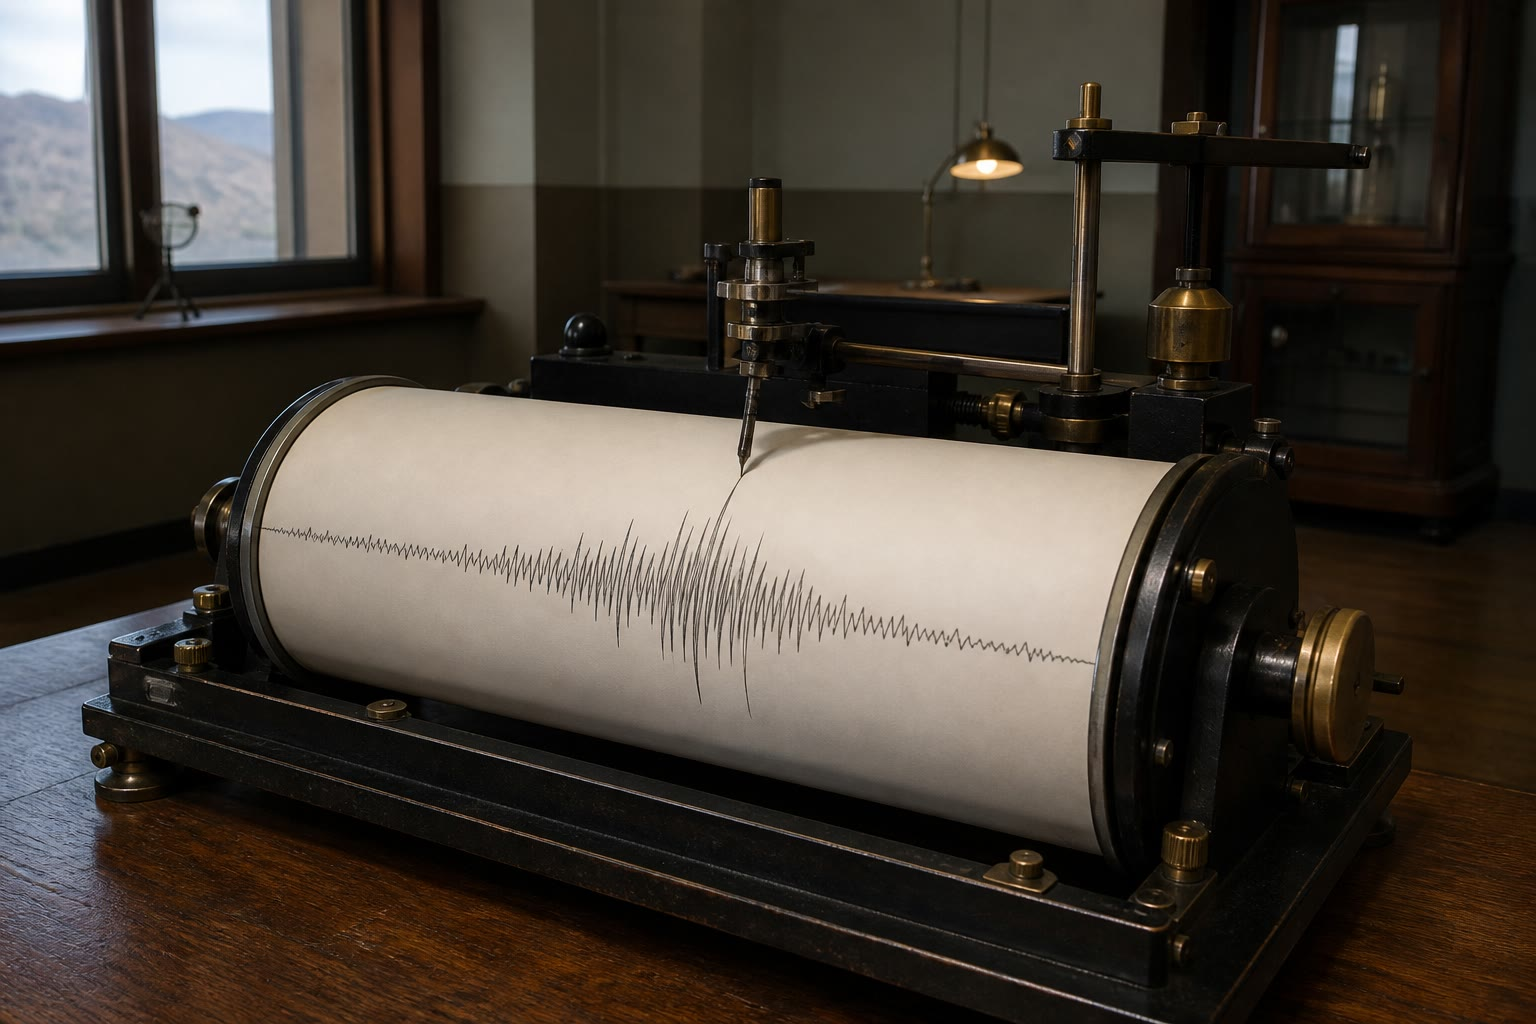
\includegraphics[width=0.58\linewidth]{images/book3/ai/b3-14-seismograph-drum.jpg}

{\small 地震仪：重物悬挂于软弹簧上，地面运动时它保持静止，笔记录下的则是两者之差——即周末问题中的底座激励振子。}
\end{omfigure}

\section{问题：地震仪}

\begin{problem}[{周末问题——一个质量块悬于弹簧上，弹簧位于
固定于地面的箱体内；地面晃动时，笔所记录的是什么，
为何同一仪器在高频时测量位移，低频时测量加速度，
以及为何长周期的
地震仪不能简单地用一根长弹簧}]
\label{pb:b1:oscillators-resonance:1}
质量 $m = \qty{1.0}{kg}$ 的物块悬挂于劲度系数为 $k$ 的弹簧上，弹簧置于
固定在地面的刚性框架内；阻尼器施加 $-\alpha\dot u$ 的力，其中
$u$ 为物块相对框架的位移，自其平衡位置量起。
地面（进而框架），
沿竖直方向移动 $x_g(t)$。远方恒星的参考系为惯性参考系。

\medskip
\noindent\textbf{第一部分——方程。}
\begin{enumerate}
  \item 将质量块的绝对位置写为 $x = x_g + u +
        \text{常量}$，在惯性参考系中列出质量块所受的力，
        并证明
        \[
        m\ddot u + \alpha\dot u + ku = -m\ddot x_g .
        \]
  \item 化为标准形式，并确定 $\omega_0$ 与 $Q$。
  \item 仪器的设计取 $f_0 = \qty{0.50}{Hz}$，$Q = 0.70$：
        求 $k$ 与 $\alpha$。
  \item 地面的恒定加速度 $a_g$（例如框架倾斜所致）
        会使 $u$ 达到何种稳态？试加以解释。
  \item 与质量块相连的笔在固定于
        框架的记录筒上书写，记录的是什么？
\end{enumerate}

\medskip
\noindent\textbf{第二部分——简谐地面运动。}
地面按 $x_g = X_g\cos\omega t$ 运动；记 $x_r = \omega/\omega_0$。
\begin{enumerate}[resume]
  \item 利用复振幅，证明 $\underline U = X_g\,x_r^2/
        (1 - x_r^2 + jx_r/Q)$。
  \item 写出 $U/X_g$ 关于 $x_r$ 与 $Q$ 的表达式。
  \item 取极限 $x_r \gg 1$，证明 $U \to X_g$，并从物理上解释
        质量块的运动（仪器测量的是什么？）。
  \item 取极限 $x_r \ll 1$，证明 $U \approx x_r^2X_g = a_g/\omega_0^2$，
        其中 $a_g$ 为地面加速度的振幅；此时的仪器
        测量的是什么？
  \item 求 $x_r = 1$ 处的值；为何 $Q \approx 0.7$ 是合理的选择？
  \item 画出 $U/X_g$ 关于 $x_r$ 的示意图（对数坐标），对 $Q = 0.7$ 与
        $Q = 5$ 两种情形。
  \item 高频时 $u$ 相对 $x_g$ 的相位为何？并加以解释。
\end{enumerate}

\medskip
\noindent\textbf{第三部分——地震仪的设计。}
远处地震产生的表面波频率为 \qty{0.05}{} 至 \qty{0.1}{Hz}，
振幅达毫米量级；局部震颤可达 \qty{5}{} 至 \qty{10}{Hz}。
\begin{enumerate}[resume]
  \item 若要将 \qty{0.05}{Hz} 的波记录为位移，需取
        $f_0 \ll \qty{0.05}{Hz}$，例如取 \qty{0.02}{Hz}。质量块的重力使弹簧产生的
        静伸长将为多少？试加以评论。
  \item 若要得到相同频率的单摆，其摆长为多少？
  \item 实际的长周期仪器采用近似水平的
        “花园门”式摆，或电子力反馈。用一句话
        解释二者各自所达到的效果。
  \item 对于 \qty{0.50}{Hz} 的仪器，计算其静伸长：
        是否可行？
  \item 用它测量频率为 \qty{0.10}{Hz}、振幅为 \qty{1.0}{mm} 的波，
        得到的 $U$ 为多少？仪器处于哪种工作区域？
  \item 一次振幅为 \qty{1.0}{mm}、频率为 \qty{5.0}{Hz} 的局部震颤：$U$ 为多少？
        属于哪种工作区域？
\end{enumerate}

\medskip
\noindent\textbf{第四部分——手机中的加速度计。}
一个由微机械加工制成、以硅弹簧支撑的质量块，其 $f_0 = \qty{1.0}{kHz}$，且
$Q = 0.7$。
\begin{enumerate}[resume]
  \item 对加速度振幅为 $g$、频率为 \qty{10}{Hz} 的抖动，计算
        $U$。此类位移如何读出？
  \item 读数在 $10\%$ 误差范围内（以 $a_g/\omega_0^2$ 为准）时，频率最高可达多少？
  \item 决定其对冲击响应的时间常数 $\tau = 2Q/\omega_0$ 是多少，
        以及为何这对探测跌落十分重要？
  \item 地震仪的 $\tau$：其数值及
        地面发生突然阶跃后的后果。
  \item 为何两种仪器都选取临界（或近临界）阻尼，
        而不取高 $Q$ 值？
  \item 手机恰在 \qty{1.0}{kHz} 处被摇晃：
        读数偏离的倍数是多少？
  \item 小结：同一个器件，两种工作区域，
        由哪一个单一的比较来决定？
\end{enumerate}
\end{problem}
